\documentclass[russian,utf8,emptystyle]{eskdtext}

\newcommand{\No}{\textnumero} % костыль для фикса ошибки

\ESKDdepartment{Федеральное государственное бюджетное образовательное учреждение высшего профессионального образования}
\ESKDcompany{Московский государственный технический университет им. Н. Э. Баумана}
\ESKDclassCode{23 0102}
\ESKDtitle{АСОИ поиска алгоритмов распознавания изоморфизма графов с помощью генетического программирования}
\ESKDdocName{Программа и методика испытаний}
%\ESKDsignature{Вариант 8Б}
\ESKDauthor{Гуща~А.~В.}
%\ESKDtitleApprovedBy{~}{~\underline{\hspace{2.5cm}}}
%\ESKDtitleAgreedBy{~}{~\underline{\hspace{2.5cm}}}
\ESKDtitleDesignedBy{Студент группы ИУ5-82}{Гуща~А.~В}
 
\usepackage{multirow}
\usepackage{longtable}
\usepackage{calc}
%\usepackage{tabularx,ragged2e}
%\renewcommand\tabularxcolumn[1]{>{\Centering}p{#1}}
\newcommand\abs[1]{\left|#1\right|}

\begin{document}
\maketitle

\section{Аннотация}
В данном документе описываются последовательность и методы проведения испытаний при тестировании программного изделия, состав и структура технических и программных средств, необходимых для проведения испытаний, а также приводятся требования к предъявляемой документации, характеристикам программы применительно к условиям эксплуатации и требования к информационной и программной совместимости.
\newpage

\tableofcontents
\newpage

\section{Объект испытаний}
Объектом испытаний является АСОИ поиска алгоритмов распознавания изоморфизма графов с помощью генетического программирования. Сокращенное название: graph-isomorph, программа, АСОИ.

\section{Цель испытаний}
Цель испытаний состоит в проверке работоспособности АСОИ и соответствия выполняемых функций требованиям документа <<Техническое задание>>.

\section{Состав предъявляемой документации}
На испытания программного продукта предъявляются следующие документы:
\begin{itemize}
\item Техническое задание
\item Программа и методика испытаний
\item Руководство пользователя
\end{itemize}

\section{Технические требования}
\subsection{Требования к программной документации}
Состав программной документации должен удовлетворять требованиям документа <<Техническое задание>>, предъявляемого по окончании работы.

Программная документация должна быть оформлена в соответствии с ГОСТ и ЕСПД по составлению и оформлению документов на программное изделие.

\subsection{Требования к техничесим характеристикам}
\subsubsection{Требования к составу аппаратного обеспечения}
Данная программа должна работать на компьютере следующей конфигурации:
\begin{itemize}
\item Процессор, поддерживающий архитектуру x86\underline{~}64 с тактовой частотой не менее 1.5 ГГц
\item Оперативная память объемом не менее 1 Гб
\item Графический ускоритель и монитор, способные отображать графический интерфейс операционной системы
\item Устройства ввода: мышь и клавиатура
\end{itemize}

\subsubsection{Требования к составу программного обеспечения}
Для работы данного приложения необходимо, чтобы на компьютере были установлены следующие программные продукты:
\begin{itemize}
\item Операционная система семейства GNU/Linux с версией ядра не ниже 3.0
\item Оконная система X Window System не ниже версии X11R7.3
\item Библиотеа элементов интерфейса GTK+ не ниже версии 3.10
\end{itemize}

\subsubsection{Требования к квалификации оператора}
Для продуктивного использования данного программного продукта пользователь должен обладать следующими навыками и знаниями:
\begin{itemize}
\item Базовые знания английского языка, если операционная система имеет английский язык как основной
\item Знания из теории графов: понятия графа, изоморфизма графов, деревья и др.
\item Базовые знания информатики: алгоритм, программа, процесс интерпретации, проблемно-ориентированный язык программирования и др.
\item Базовые знания эволюционных методов: функция приспособленности, популяция, индивиды, геном и др.
\end{itemize}

\section{Состав и порядок испытаний}
Испытания данного программного продукта должны проводиться в следующем порядке:
\begin{itemize}
\item Инсталляция АСОИ. Установка программного изделия осуществляется в соответствии с руководством пользователя (см. документ руководство пользователя, пункт 3.1)
\item Запуск АСОИ. Запуск программного изделия осуществляется в соответствии с руководством пользователя (см. документ руководство пользователя, пункт 3.2)
\item Тестирование базовых операций АСОИ
\end{itemize}

\subsection{Требования к составу аппаратного обеспечения}
Требования к составу аппаратного обеспечения учитываются согласно документу программа и методика испытаний, пункт 5.2.1.

\subsection{Требования к составу программного обеспечения}
Требования к составу программного обеспечения учитываются согласно документу программа и методика испытаний, пункт 5.2.2.

\newpage
\section{Методы испытаний}
~\\
\begin{longtable}{
  p{0.7cm}|p{1.5cm}|p{6.5cm}|p{6.5cm}
}

№ & Пункт ТЗ & Выполняемые действия & Результат \\ \hline 
\endhead

1 & 5.2.а & Окно настроек: выбрать оператор в списке в левой части окна. & Отображение имени и описание оператора в центральной части окна (См приложение рис.~\ref{fig:optionsWnd}). \\ 
\hline 

2 & 5.2.б & Окно настроек: & \\
  &       & 1. выбрать поле ввода параметра в правой части окна из списка. Просмотреть текущее значение параметра. & Подсведка поля ввода (рис.~\ref{fig:parSelect}) \\
\cline{3-4}
  &       & 2. Ввести новое значение параметра. Перевести фокус на другое поле ввода. & В случае успеха значение поле изменится, в случае ошибки проверки входных данных будет отображен диалоговое сообщение с текстом ошибки (рис.~\ref{fig:parSelectError}). \\
\hline

3 & 5.2.в & Любое окно: & \\
  &       & 1. Активировать в главном меню <<Файл>> пункт <<Сохранить проект как>> & Откроется диалоговое окно сохранения проекта (рис.\ref{fig:projectSaveDialog}). \\
\cline{3-4}
  &       & 2. Выбрать название файла. Нажать <<ОК>>. Просмотреть папку с файлом. & По абсолютному пути сохранения проекта появился выбранный файл (рис.~\ref{fig:projectSaveResult}). \\
\cline{3-4}
  &       & 3. Активировать в главном меню <<Файл>> пункт <<Открыть проект>> & Откроется диалоговое окно открытия проекта (рис.~\ref{fig:projectOpenDialog}). \\
\cline{3-4}
  &       & 4. Выбрать сохраненный ранее файл проекта и нажать на <<ОК>>. Проверить загруженные данные. & Параметры эволюции и популяция обновятся в соответствии с загруженными данными. \\
\hline

4 & 5.2.г & 1. Открыть окно эволюции: активировать меню <<Вид>> пункт <<Показать окно эволюции>> & На экране появится окно эволюции (рис.~\ref{fig:evolutionWndFresh})\\
\cline{3-4}
  &       & 2. Нажать на кнопку запуска эволюции (кнопка с черным треугольником). & Изображения входных графов начинают меняться, статус процесса в нижнем горизонтальном индикаторе выполнения увеличивается (см. рис.~\ref{fig:evolutionWndStartPause}). \\
\cline{3-4}
  &       & 3. Нажать на кнопку паузы эволюции (кнопка с двумя вертикальными прямоугольниками). & Изображения входных графов больше не меняются, статус процесса в нижнем горизонтальном индикаторе выполнения не увеличивается (см. рис.~\ref{fig:evolutionWndStartPause}). \\
\cline{3-4}  
  &       & 4. Нажать на кнопку запуска эволюции. & Изображения входных графов начинают меняться, статус процесса в нижнем горизонтальном индикаторе выполнения увеличивается (см. рис.~\ref{fig:evolutionWndPauseStart}). \\
\cline{3-4} 
  &       & 5. Нажать на кнопку остановки эволюции (кнопка с черным квадратом). & Статус процесса сбрасывается в ноль процентов (см. рис.~\ref{fig:evolutionWndStop}). \\
\hline

5 & 5.2.д & 1. Открыть окно эволюции: активировать меню <<Вид>> пункт <<Показать окно эволюции>> & На экране появится окно эволюции (рис.~\ref{fig:evolutionWndFresh})\\
\cline{3-4}
  &       & 2. Нажать на кнопку запуска эволюции. & Изображения входных графов начинают меняться (см. рис.~\ref{fig:evolutionWndStartPause}). \\
\cline{3-4}
  &       & 3. Нажать на кнопку паузы эволюции. Проанализировать изображения входных графов. & Изображения входных графов больше не меняются, можно проводить анализ входных данных (см. рис.~\ref{fig:evolutionWndStartPause}). \\
\hline

6 & 5.2.e & 1. Открыть окно эволюции: активировать меню <<Вид>> пункт <<Показать окно эволюции>> & На экране появится окно эволюции (рис.~\ref{fig:evolutionWndFresh})\\
\cline{3-4}
  &       & 2. Нажать на кнопку запуска эволюции. & Изображения входных графов начинают меняться (см. рис.~\ref{fig:evolutionWndStartPause}). \\
\cline{3-4}
  &       & 3. Ждать, пока не обработается одно поколение (индикатор прогресса дойдет до 100\% и сбросится в 0\%). Нажать на кнопку паузы эволюции. Проанализировать промежуточные результаты. & Значения в полях промежуточных значений обновились (см. рис.~\ref{fig:evolutionWndNextGeneration}). \\
\hline

7 & 5.2.ж & 1. Открыть окно эволюции: активировать меню <<Вид>> пункт <<Показать окно эволюции>> & На экране появится окно эволюции (рис.~\ref{fig:evolutionWndFresh})\\
\cline{3-4}
  &       & 2. Нажать на кнопку запуска эволюции. & Статус процесса в нижнем горизонтальном индикаторе выполнения увеличивается (см. рис.~\ref{fig:evolutionWndPauseStart}). \\
\hline

8 & 5.2.з & 1. Выполнить действия в пункте №5. Открыть окно результатов: активировать меню <<Вид>> пункт <<Показать окно результатов>> & На экране появится окно результатов (рис.~\ref{fig:resultsWnd})\\
\cline{3-4}
  &       & 2. Просмотреть список алгоритмов-индивидов в левой части окна, выбрать одного индивида щелчком по его имени. & Центральная и правая часть окна обновятся и будут отображать текстовое и графическое представление исходного кода соответственно (см. рис.~\ref{fig:resultsWndSelectInd} и рис.~\ref{fig:resultsWndGraphInd}) \\
\end{longtable} 

\newpage
\section{Приложение}

\begin{figure}[h!]
\centering
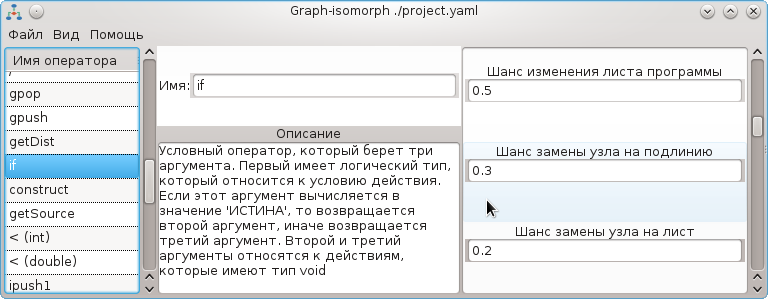
\includegraphics[width=0.9\textwidth]{screen07}
\caption{Окно настроек}
\label{fig:optionsWnd}
\end{figure}

\begin{figure}[h!]
\centering
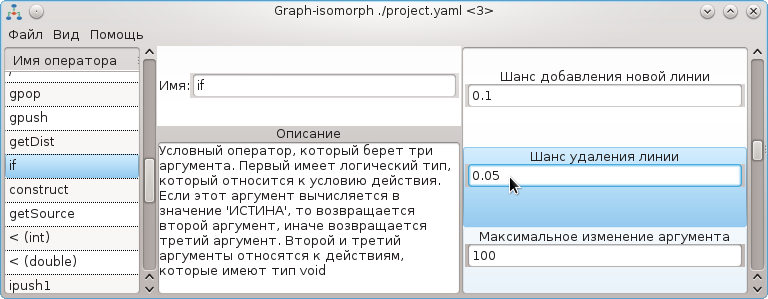
\includegraphics[width=0.9\textwidth]{screen12}
\caption{Просмотр параметра эволюции}
\label{fig:parSelect}
\end{figure}

\begin{figure}[h!]
\centering
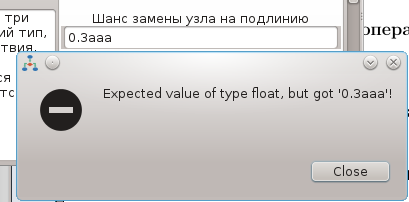
\includegraphics[width=0.5\textwidth]{screen08}
\caption{Сообщение об ошибке распознавания входных данных}
\label{fig:parSelectError}
\end{figure}

\begin{figure}[h!]
\centering
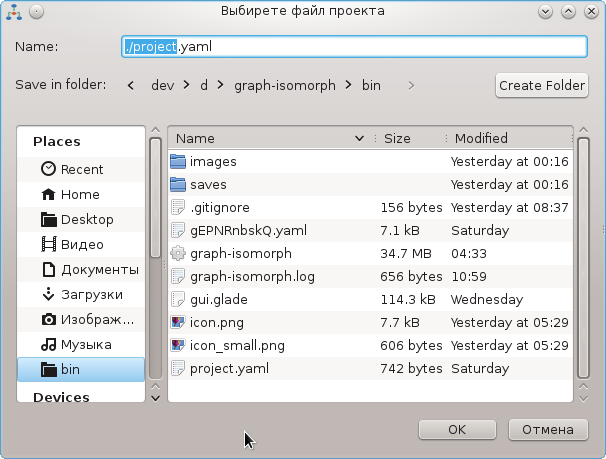
\includegraphics[width=0.8\textwidth]{screen06}
\caption{Диалог cохранения проекта}
\label{fig:projectSaveDialog}
\end{figure}

\begin{figure}[h!]
\centering
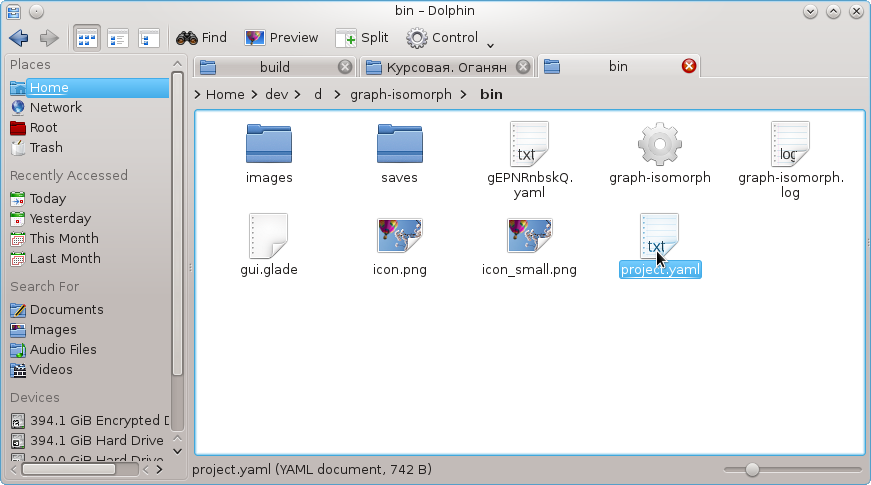
\includegraphics[width=0.8\textwidth]{screen13}
\caption{Файл проекта в файловом менеджере}
\label{fig:projectSaveResult}
\end{figure}

\begin{figure}[h!]
\centering
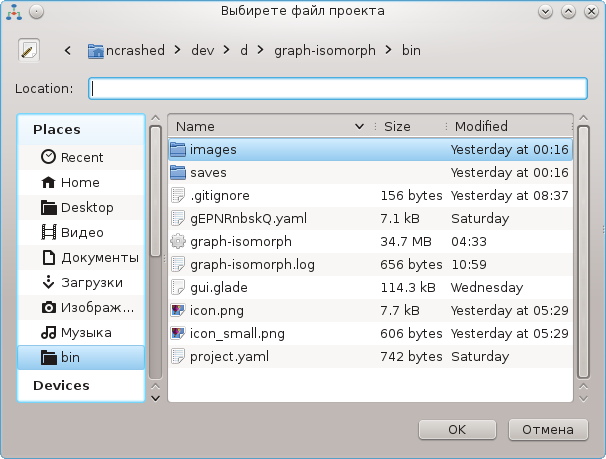
\includegraphics[width=0.8\textwidth]{screen05}
\caption{Диалог открытия проекта}
\label{fig:projectOpenDialog}
\end{figure}

\begin{figure}[h!]
\centering
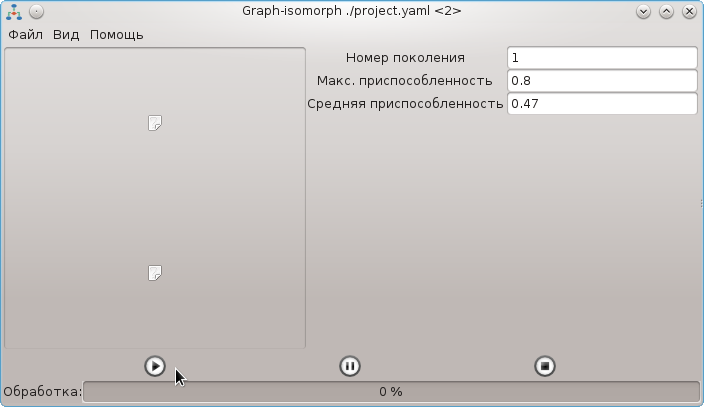
\includegraphics[width=0.8\textwidth]{screen14}
\caption{Только что открытое окно эволюции}
\label{fig:evolutionWndFresh}
\end{figure}

\begin{figure}[h!]
\centering
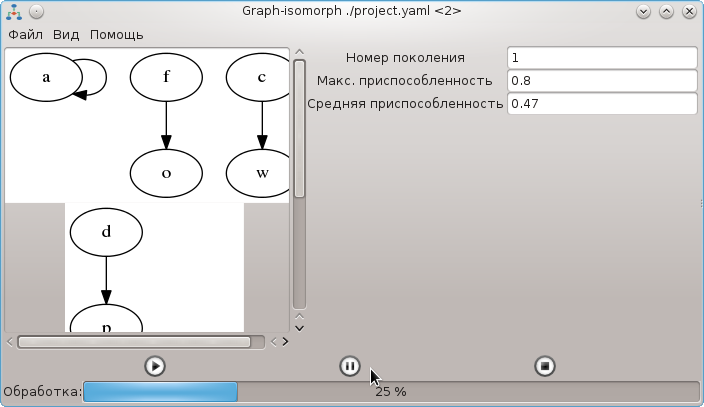
\includegraphics[width=0.8\textwidth]{screen15}
\caption{Запуск эволюции и постановка на паузу}
\label{fig:evolutionWndStartPause}
\end{figure}

\begin{figure}[h!]
\centering
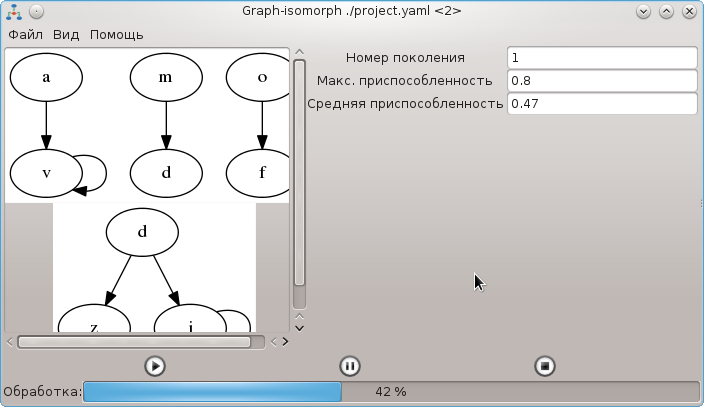
\includegraphics[width=0.8\textwidth]{screen16}
\caption{Возобновление эволюции}
\label{fig:evolutionWndPauseStart}
\end{figure}

\begin{figure}[h!]
\centering
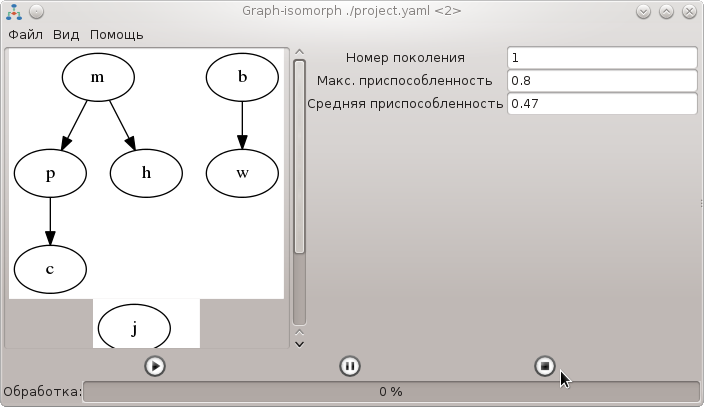
\includegraphics[width=0.8\textwidth]{screen17}
\caption{Остановка эволюции}
\label{fig:evolutionWndStop}
\end{figure}

\begin{figure}[h!]
\centering
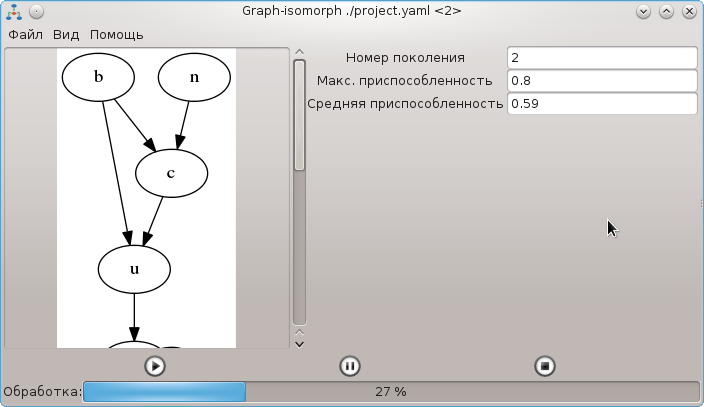
\includegraphics[width=0.8\textwidth]{screen18}
\caption{Обновление промежуточных результатов}
\label{fig:evolutionWndNextGeneration}
\end{figure}

\begin{figure}[h!]
\centering
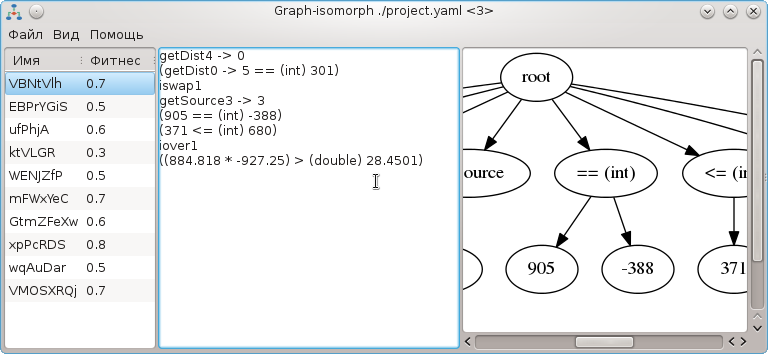
\includegraphics[width=0.8\textwidth]{screen19}
\caption{Окно результатов}
\label{fig:resultsWnd}
\end{figure}

\begin{figure}[h!]
\centering
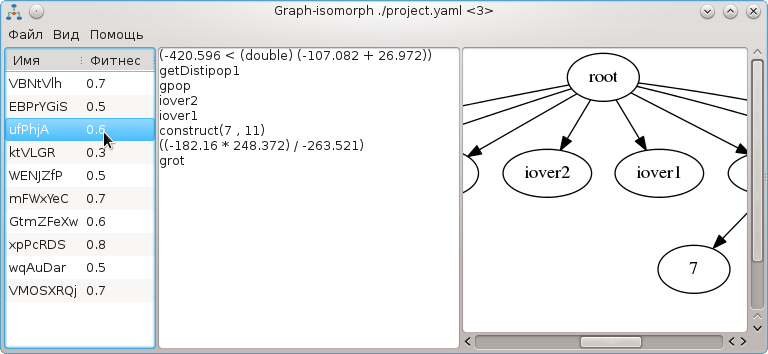
\includegraphics[width=0.8\textwidth]{screen20}
\caption{Выбор одного из текущих алгоритмов и просмотр его значения функции приспособленности и его исходного кода}
\label{fig:resultsWndSelectInd}
\end{figure}

\begin{figure}[h!]
\centering
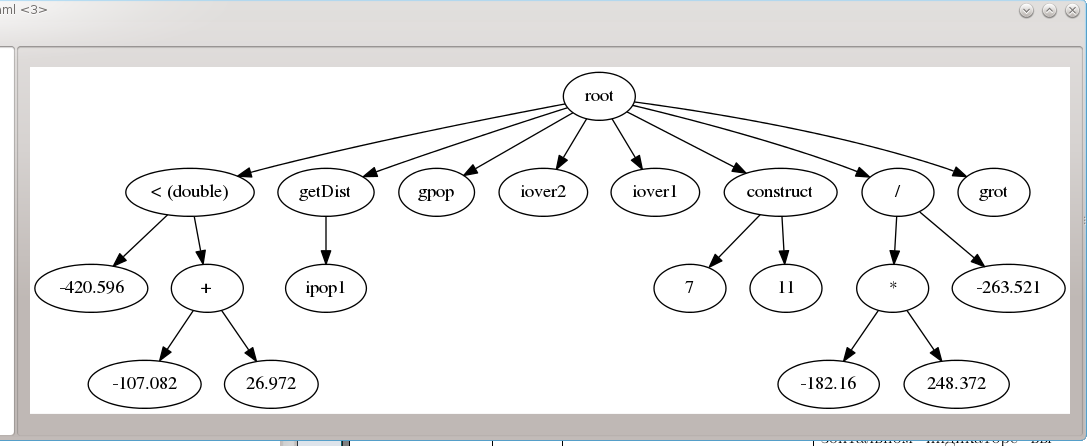
\includegraphics[width=0.8\textwidth]{screen21}
\caption{Просмотр графической формы исходного кода индивида}
\label{fig:resultsWndGraphInd}
\end{figure}
\end{document}


